\section{Practical Sentiment Analyse}
\label{sec:sent}
\par The main purpose of sentiment analyse is to discover views and opinions diversity \cite{katiyar2016investigating} of different targets in films which reflect what attract audience watching the movie. The sample dataset in this area are review corpus $ R =\{r_1, r_2, \dots, r_n\}$ and each $r_i$ has film name  $f_i$ it belonging to, time point $time_i$ , scores towards this film $s_i$ and user $u_i$ who scores. These attributes of reviews are discrete (has domain specific value) and many sentences in it contribute to the whole sentiment of this single review. Since reviews are spread in social media platform such as twitter or micro-blogs, the sentences are limited and review of movie are usually enough short. Thus, many phenomenon occurred on short texts or natural language add difficulties when analysing the sentiments of targets (e.g. Rhetoric, metaphor, proverb and nicknames)\cite{li2014sentiment}. Unlike many works focus on proceed in sentence-level document-level and time-period level step by step\cite{chen2017improving}, we try to figure out the sentiment to a specific actors or director(leading creator of this film)\cite{dong2014adaptive}. A useful prior knowledge in reviews together with reviewers' rating score or stars made by user is evaluation score of specific film. We make the best of this knowledge to enlarge our sentiment words database because user usually behave consistent sentiment to same target.

\subsection{Named Entities Recognition}
\par If we want to know sentiments behind human expression, targets that people are taking about should be identified firstly. Here we concentrate on comment target about leader creators in films. The main challenging is the nicknames for actors and directors.
\par \textbf{Sequence to sequence approach}. Given a word sequence $X=\{x_1, x_2, \dots, x_n\}$ we observed and the 4-tag label set $Tags=\{O,B,E,M\}$, the objective task is to find correct corresponding labels $Y=\{y_1, y_2, \dots, y_n | y_i \in Tags\} $. By optimizing the loss function with parameter $ \theta $
\begin{equation}
    J(\theta)= \arg\min_{\theta} \frac{1}{n}\sum_{i=1}^{n}loss(f(x_i;\theta), y_i)
\end{equation}
recurrent neutral networks such as \emph{LSTM}, \emph{BidirectionalLSTM}, \emph{BidirectionalLSTM+CRF} \cite{chen2017improving} have been proved to be state-of-art structures. They consider both long time and short terms information and find tags with maximum possibility for sequence labeling. However, previous machine learning approaches need huge domain training data, while it is hardly to label these social media corpus accurately which are full of informality and flexibility. Especially actors get constantly evolving new roles in various films as time goes by, we hope find a simple and efficient way that recognize most of the comment targets in films reviews.
\par \textbf{Fast and adaptive approach}. In order to mining entities in linear time, we apply key word matching for leader creators in films. Online knowledge database which store film meta information can be strong support providing comprehensive and dependable analysis. Focused crawling technology based on web linkage contribute to construction of prior knowledge of \textbf{actors}, \textbf{roles} and \textbf{directors}.

\begin{algorithm}[htb]
\renewcommand{\algorithmicrequire}{\textbf{Input:}}
\renewcommand\algorithmicensure {\textbf{Output:} }
\caption{ Framework of nickname mining for our system}

\begin{algorithmic}[1]

\REQUIRE ~~\\
The name set of \textbf{actors} and \textbf{directors} in each film\\
The name set of \textbf{roles} for each actors used to played\\
Threshold $\boldsymbol\alpha$ for minim similarity of misspell and variation\\
Threshold $\boldsymbol\beta$ for max tolerance of misspell and variation\\

\ENSURE ~~\\
Potential comment targets mapping dictionary $A$, $P$\\

\STATE Aggregating reviews group by corresponding film name along with preparing actors list $A_i$, directors list $P_i$ in $i$th film according given \textbf{actors} and \textbf{directors};
\STATE Constructing actors mapping $A$ for every actor in $ a_i$, so dose $P$ for every director in $p_i$;
\STATE Quality similarity between every noun morphemes $w$ and $t$ in \textbf{roles}, \textbf{actors} and \textbf{directors} by \emph{Jaccard} char distance in all comments for one film;
\STATE Recognizing potential nickname by the similarity and threshold $\boldsymbol\alpha$ we set, if $Jaccard(w, t) > \alpha$ add it to mapping dictionary $A$ or $P$;
\STATE Checking potential nickname in mapping dictionary, if $Levenshtein(w, t) > \beta $, delete it from mapping dictionary $A$ or $P$;
\RETURN $A$, $P$

\end{algorithmic}
\label{alg:ner}
\end{algorithm}

\begin{table*}[!t]
\begin{center}
  \centering
  \begin{tabular}{|c|c|c|c|c|c|c|}
    \hline
    Review No. & Contents & Referred & Film No.& time point  & Scores \\
    \hline
    1 & \tabincell{l}{Yang Yang's hard temperament\\ is enough to hold up the role} & Yang Yang & Ten great II of peach blossom & 2016-07-25T13:36:12.000+0800 & 10\\
    2 & \tabincell{l}{Yang Yang's acting is really \\ embarrassing, Crystal Liu is OK} & \tabincell{l}{Yang Yang,\\ Crystal Liu}& Ten great II of peach blossom & 2017-08-07T20:18:55.000+0800 & 5\\
    3 & \tabincell{l}{The story of embarrassment,\\ feeling Yehua did not love Baiqian} & \tabincell{l}{Yang Yang,\\ Crystal Liu} &  Ten great II of peach blossom & 2017-08-07T21:09:07.000+0800 & 2\\
    $r_i$ & \dots & \dots & $f_i$ & $time_i$  & $s_i$ \\
    \hline
  \end{tabular}
  \caption{review targets after named entities recognition}
\end{center}
\label{tab:summary}
\end{table*}

\par Assume average noun morphemes length is $m$ for all $n$ reviews and $t$ targets for all $F$ films. Algorithm \ref{alg:ner} need compare $ c \times nmt$ times. Since word comparing consume limited space and time and $ m \ll n, t \ll n $, we extract potential comment targets in $ O(n) $ time complexity which greatly less than deep learning approach. We can easily adjust designed parameter and improve efficiency with parallel framework when processing TB data.

\par In order to decrease the storage space of data, we replace film name and user name by mapping them using film id and user id. $f_i \in F=\{f_1, f_2, \dots, f_m\}$ and $u_i \in U = \{u_1, u_2, \dots, u_U\}$. Let score for each review be $s_i \in [0, 10]$ and $time_i$ be the timestamps. The features we finally retrieved can be summarized in table \ref{tab:summary}.

\subsection{Target-Dependent Sentiment Classification}
\par Sentences tend to be more complex when targets we want to analyse increase and sentiments detection being a hard work when analysing more objects. We take leader creator of film as major targets in this paper. Examples containing multi targets are shown as follows.
\begin{enumerate}
  \item Live here now! The point of life is looking for the point. ---\emph{A dog's purpose}
  \item It has been a year since I were familiar with Alexander Sandro Gonzalez Inarritu whose films have a cruel irony and full bitterness.---\emph{Bird man}
  \item Mia had dreamed of becoming an actress known by more audience, while Sebastian want to won a place in his loving jazz. ---\emph{LaLa land}
\end{enumerate}
\par  Sentence(1) is a non-target review, while Sentence(2) shows one-target sample and Sentence(3) stands for multi-target sentences. Considering targets after NER process in section 4.1 consist of actors map list $A=\{a_1, a_2, \dots, a_A\}$ and directors map list $P=\{p_1, p_2, \dots, p_P\}$, we cluster sentences into comments set with two polarity(positive $+1$ and negative $-1$). Binary sentiment classifier play an important role in sentiment classification. Sentiment polarity $SP=\{+1, -1\}$ labeled by classifier for each sentences in corpus $st_i^j$ of $i$th film with corresponding target $j$, $j \in A \cup P $ and targets capacity $T = ||A||+||P||$. Let $T_i$ be number of targets in film $i$. We try to find out following segments.

\begin{equation}
    Neg=\bigcup_1^{F} ng_i \ | \ polarity \ of \ ng_i = -1, \ ng_i \in \bigcup_{j=1}^{T_i} st_i^j
    \label{eq:neg}
\end{equation}
\begin{equation}
    Pos=\bigcup_1^{F} ps_i \ | \ polarity \ of \ ps_i = +1, \ ps_i \in \bigcup_{j=1}^{T_i} st_i^j
    \label{eq:pos}
\end{equation}

\par Since we have to retrieve \emph{Neg} and \emph{Pos} shown in Equation (\ref{eq:neg}) and (\ref{eq:pos}), we take training data $R_p$ with scores larger than 9 for positive sentiment and $R_n$ which scores lower than 3 for negative one. We exclude reviews $R_{ambi}$ which scores range between 4 and 8 that might be ambiguous over sentiment in training phrase. Instead, $R_p$ and $R_n$ show more concentrated sentiments in words. We train a classifier on $R_p$ and $R_n$, then we split $R$ with context window according referred target in each review. Reviews segments cover target's contextual information which construct sentiment corpus $Neg$ and $Pos$ towards specific targets are objectives for sentiment classifier. We mainly apply it on targets segments split from $R_{ambi}$. Finally, we get comprehensive sentiment polarity on targets segments in $R$.

\par Lexicon based sentiment analysis is constrained by sentence structure, latent word meaning and confused word features. We introduce bidirectional long short term memory (\emph{Bi-LSTM}) neural network \cite{tang2015target-dependent,chen2017improving} for end-to-end sentiment classification and automated feature learning as figure \ref{fig:lstm} shows.

\begin{figure}[!htbp]
\centering
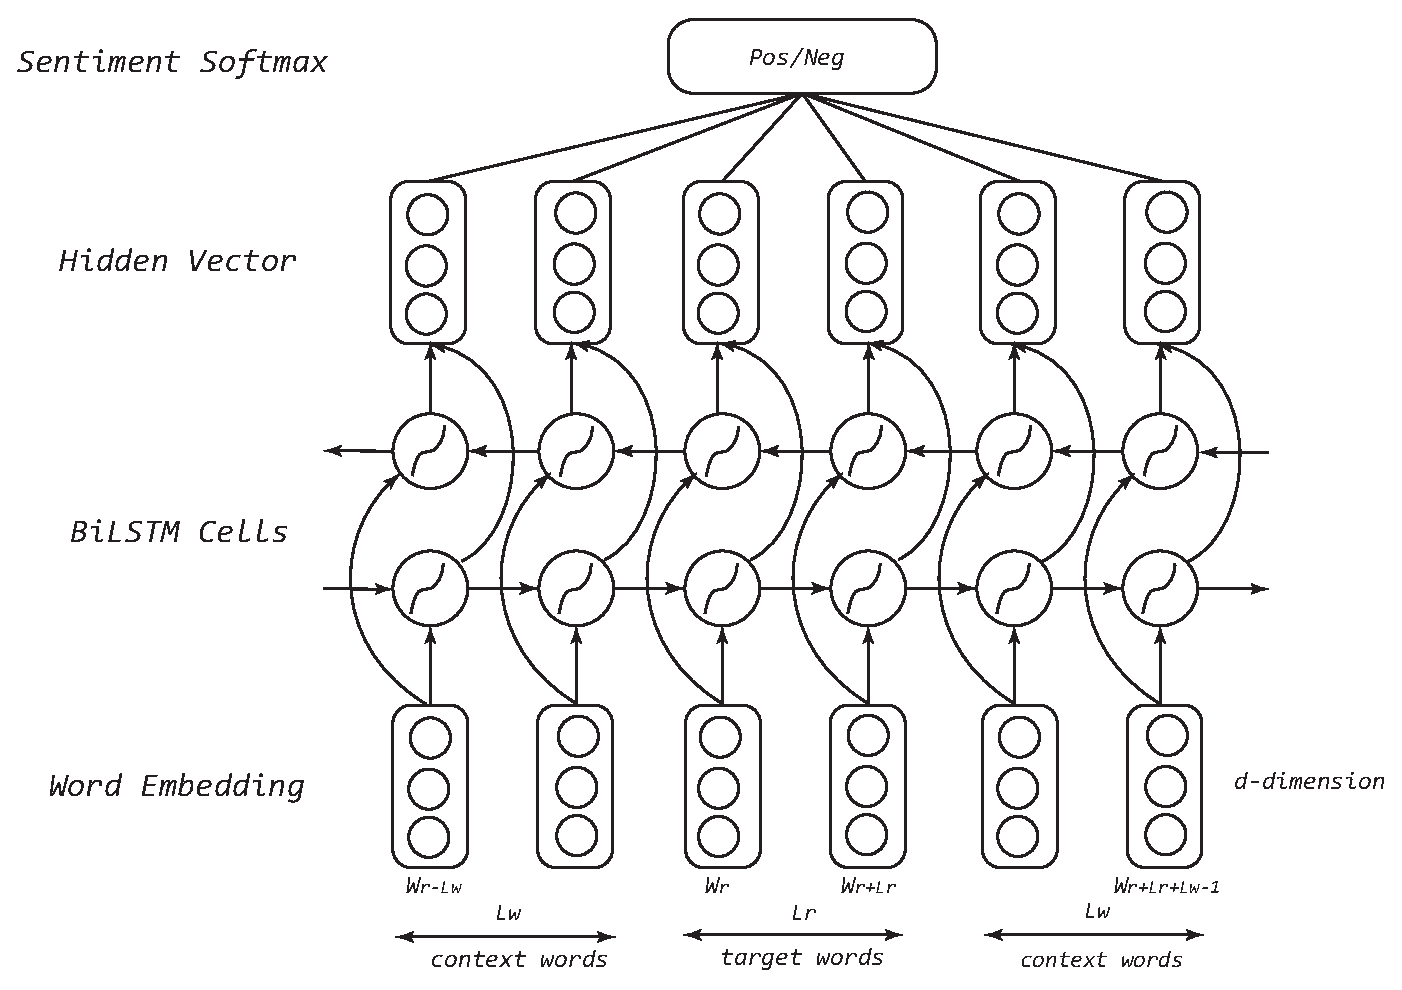
\includegraphics[width=\columnwidth]{bi-lstm.eps}
\caption{Structure of Bi-LSTM Sentiment Classifier, where $L_r$ for target words length and $L_w$ for context length we extract from original sentence. First layer in Bi-LSTM stands for forward hidden layer and the second layer are the backward one.}
\label{fig:lstm}
\end{figure}

\par Specially, word sequence are represented as a low dimensional , continuous and valued vector. It is called word embedding and we use pre-trained vectors so as to make better use of semantic and grammatical associations. Assume each $d$-dimension vector $ W_i = \mathbb{R}^{d \times |V|}$ for $i$th word in whole vocabulary $V$. Targets words with $L_r$ length cover $tw = \{W_r, W_{r+1}, \dots, W_{r+L_r-1}\}$ and context words $cw = \{W_{r-L_w}, \dots, W_{r-1}, W_{r+L_r}, \dots, W_{r+L_r+L_w-1}\}$ with window length $L_w$ surround corresponding targets words $tw$. \emph{BiLSTM} maps word vectors to fix-length sentence vector by recursively transformation above vectors of previous time step $h_{t-1}$. Cells for \emph{BiLSTM} in Figure \ref{fig:lstm} contains neural gates: input gates, forget gates, and output gates which adaptively remember input vector, forget history, and generate output vector. We add softmax layer to output sentiment of sentence vector which cover hidden representation of vectors for specific target segment as Figure 1 shows. Core calculation in LSTM cells are listed in bellow equations. \cite{} $\odot$ is element-wise multiplication and $\sigma$ is sigmoid activation, $W_i, W_f, W_o, b_i, b_f, b_o$ are parameters for input, forget and output gates.
\begin{subequations}
\begin{align}
  i_t &= \sigma(W_i \bullet [h_{t-1};w_t] + b_i)\\
  f_t &= \sigma(W_f \bullet [h_{t-1};w_t] + b_f)\\
  o_t &= \sigma(W_o \bullet [h_{t-1};w_t] + b_o)\\
  g_t &= \tanh(W_r \bullet [h_{t-1};w_t] + b_r)\\
  c_t &= i_t \odot g_t + f_t \odot c_{t-1}\\
  h_t &= o_t \odot \tanh(c_t)
\end{align}
\end{subequations}


\subsection{Film-level Sentiment Trend}
\par In this section, we mainly care about how to predict latent sentiment transform. Obviously, we quantify explicit sentiment towards special actors or directors. Although all information came from overall corpus, we can not deny that different sentiment exist in different time period during movie life. Audience's sentiments have trends and always behave dynamically. Previous work concentrate on sentiment polarity and we extend it by capture dynamic time-period sentiment. Denote a time period range from $time_r = [time_i, time_j]$, we capture review statistical sum $R_{f_i}$ of each movie $f_i$ at time period $time_r$ from $Pos$ and $Neg$. Then we get different target $j$'s positive or negative sentiment transformation at different $time_r$.

\begin{equation}
    SentimentPos^j_i (time_r) = 10\cdot \frac{|pos^j_i \ in \ time_r|}{R_{f_i}}
\end{equation}

\begin{equation}
    SentimentNeg^j_i (time_r) = 10\cdot \frac{|neg^j_i \ in \ time_r|}{R_{f_i}}
\end{equation}

\par Dynamic sentiment on leader creator shows how people transform their attention from different targets in movies. We pick out most interesting part (actor) from them and label it the main factor which mainly contribute to the box-office of specific film. The trend analyse is shown in Figure \ref{fig:sentiment}.

\par To measure the smoothness of the sentiment time series, we use slice window to capture the changes in the emotional inclination of the reviews. We Denote upper bound and lower bound of a day $r$,$UBP^j_i (r)$, $LBP^j_i (r)$,$UBL^j_i (r)$ and $LBN^j_i (r)$.

\begin{equation}
    UBP^j_i (r) = mean^j_i (time_r)+\lambda \cdot std^j_i (time_r)
\end{equation}

\begin{equation}
    LBP^j_i (r) = mean^j_i (time_r)-\lambda \cdot std^j_i (time_r)
\end{equation}

where
\begin{equation}
    mean^j_i (r) = \frac{1}{2d}\sum_{k=r-d}^{r+d}SentimentPos^j_i (time_k)
\end{equation}

\begin{equation}
    std^j_i (r) = \frac{1}{2d}\sum_{k=r-d}^{r+d}(SentimentPos^j_i (time_k)- mean^j_i (time_r))^2
\end{equation}

\par Because the time series follows Gaussian Distribution, and we set $\lambda=2$, means that confidence intervals is 0.0456,

\begin{figure}[!htbp]
\centering
\subfloat[Period Sentiment Trend: Change of sentiment in a specific film]{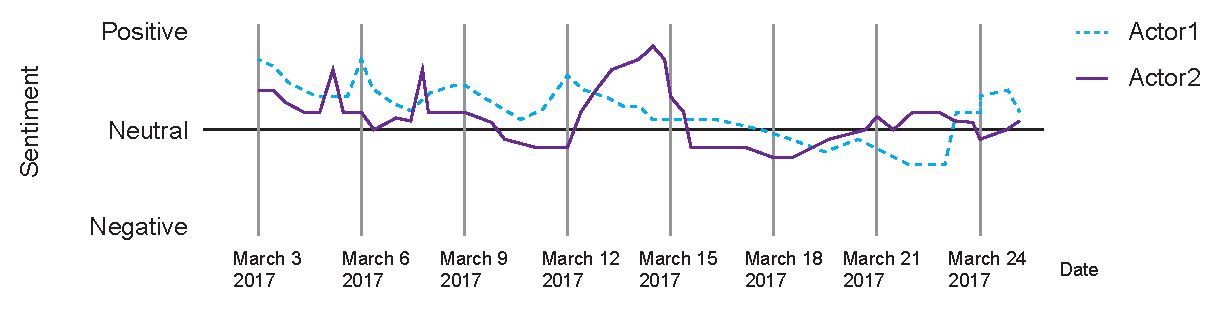
\includegraphics[width=\columnwidth]{sentiment_1.eps}}
\hfill
\subfloat[Dynamic Sentiment on Leader Creator : General sentiment transform of an actor in past five years]{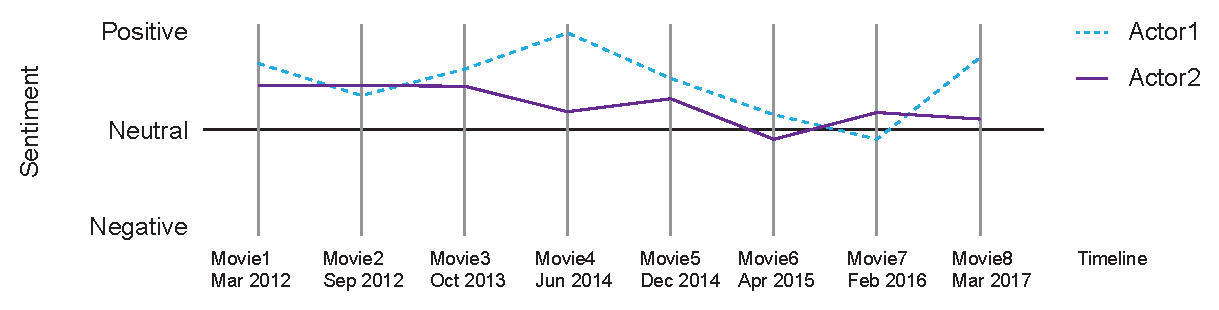
\includegraphics[width=\columnwidth]{sentiment_2.eps}}
\caption{Film-level sentiment trend analyse of different time period. a) shows the change of sentiment in one film life period which indicates what attract people. b) shows the average sentiment of a specific actor which indicates highest moments and lowest moment of an actor career }
\label{fig:sentiment}
\end{figure}


